\documentclass[10pt,t]{beamer}
\usepackage{pslatex}
\usepackage{fontspec}
\newfontfamily\DejaSans{DejaVu Sans}
\usepackage{caption}
\usepackage{subcaption}
\usepackage{ amssymb }
\usepackage{amsmath}
\usepackage{semantic}
\newcommand*{\defeq}{\stackrel{\text{def}}{=}}
\usetheme[nat,dogma,totalframes=show]{Frederiksberg}

\usepackage{listings}
\usepackage{xcolor}

\definecolor{codegreen}{rgb}{0,0.6,0}
\definecolor{codegray}{rgb}{0.5,0.5,0.5}
\definecolor{codepurple}{rgb}{0.58,0,0.82}
\definecolor{backcolour}{rgb}{0.95,0.95,0.92}

\lstdefinestyle{mystyle}{
    backgroundcolor=\color{backcolour},
    commentstyle=\color{codegreen},
    keywordstyle=\color{magenta},
    numberstyle=\tiny\color{codegray},
    stringstyle=\color{codepurple},
    basicstyle=\ttfamily\tiny,
    breakatwhitespace=false,
    breaklines=true,
    captionpos=b,
    keepspaces=true,
    numbers=left,
    numbersep=5pt,
    showspaces=false,
    showstringspaces=false,
    showtabs=false,
    tabsize=2,
    texcl=false
}

\lstset{style=mystyle}
\usepackage{changepage}
\usepackage{ebproof}
\newcommand{\lra}[1]{\langle #1 \rangle}
\newcommand{\tycheck}[2]{#1 \Leftarrow #2}
\newcommand{\synth}[2]{#1 \Rightarrow #2}
\newcommand{\contextcons}[1]{\Gamma,#1\vdash_{\Sigma}}
\newcommand{\context}{\Gamma\vdash_{\Sigma}}
\newcommand{\vdashs}{\vdash_\Sigma}
\newcommand{\nilsig}{\langle\rangle}
\newcommand{\subst}[3]{[#1/#2]#3}
\newcommand{\judge}[4]{\sigma_{#1};#2 \downarrow #3;\sigma_{#4}}
\newcommand{\pilf}[3]{\Pi #1 : #2. #3}

\title{Proof checking in the Linux kernel}
\subtitle{}
\author{Jacob Herbst (mwr148)}
\institute[DIKU]{Institute of Computer Science (DIKU)}
\date[]{\today}

\begin{document}
\frame[plain]{\titlepage}

\begin{frame}[c]
  \begin{center}
  \frametitle{Agenda}
  \begin{itemize}
    \item eBPF, Proof Carrying Code and why we need a proof-checker in the kernel
    \item Logical Framework with Side Conditions (LFSC)
    \item An LF proof
    \item Shortcomings of the implementation
    \item Conclusion
  \end{itemize}
\end{center}
\end{frame}

\begin{frame}[containsverbatim]
  \frametitle{eBPF and why we want formal verification}
  \begin{itemize}
    \item eBPF is a virtual machine that gives sandbox functionality with kernel privileges.
    \item limbo between usability and safety
    \item programs are checked by static analysis called the eBPF verifier.
          \begin{itemize}
            \item 19k lines of code.
            \item many bugs, making eBPF security hazard
            \item disabled by default in most Linux distributions.
          \end{itemize}
  \end{itemize}
  \begin{figure}
    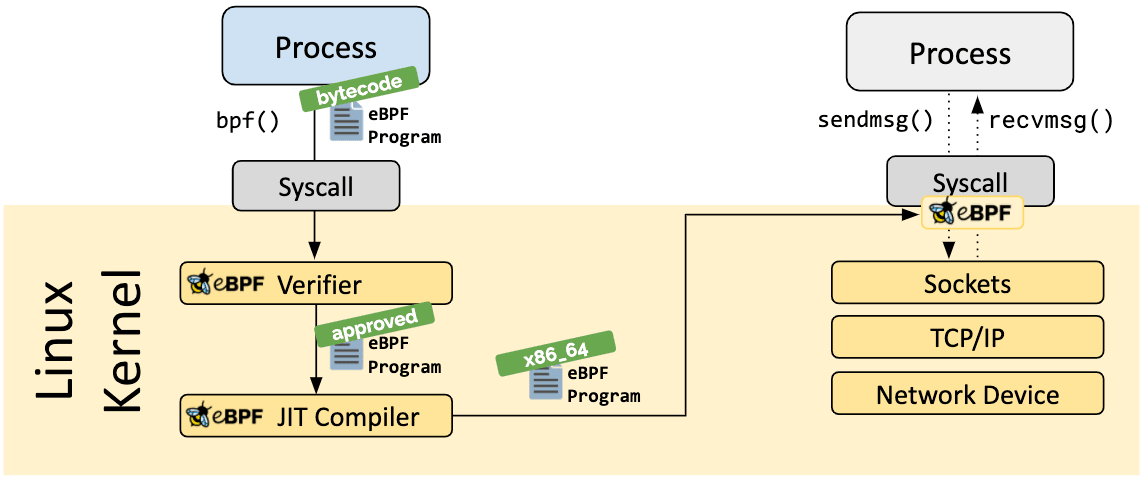
\includegraphics[width=.65\linewidth]{loader.png}
    \caption{Loading process of eBPF\footnote{\url{https://ebpf.io/what-is-ebpf/}} }
  \end{figure}
\end{frame}

\begin{frame}[c]
  \frametitle{Proof Carrying Code}
  \begin{columns}[onlytextwidth]
    \begin{column}{0.4\textwidth}
      \begin{itemize}
        \item code producer is responsible for ensuring the correctness
        \item code consumer shall check that proofs have not been tampered and
              that a certificate is valid.
      \end{itemize}
    \end{column}
    \hfill
      \begin{column}{0.6\textwidth}
      \begin{figure}
        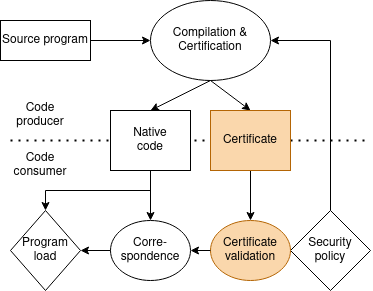
\includegraphics[width=\textwidth]{pccimg.png}
        \caption{Structure of PCC}
      \end{figure}
    \end{column}
  \end{columns}
\end{frame}

\begin{frame}[c]
  \frametitle{Logical Framework - with Side Conditions?}
  \begin{itemize}
    \item An extension of the simply typed lambda calculus with dependent product type
          \begin{itemize}
            \item $\prod_{x: A} B(x)$, with $A : \mathcal{U}$ and $B : A \rightarrow \mathcal{U}$
            \item if $x \notin FV(B)$ then $A \rightarrow B$
          \end{itemize}
    \item Used for computer-assisted proofs using the Curry-Howard correspondence % types are propositions and programs are proofs of a type since they inhabit the type.
          \begin{tabular}{c|c}
Formal Logic & Type Theory\\
\hline
$\top$ (true) & () \\
$\bot$ (false) & void \\
$\wedge$ (conjunction) & product type \\
$\vee$ (disjunction) & sum type \\
$\rightarrow$ (implication) & function type\\
$\forall$ (universal quantification) & \Pi (dependent type) \\
          \end{tabular}
    \item LFI extend LF with implicit arguments
    \item LFSC extend LFI with Side Conditions
  \end{itemize}
\end{frame}

\begin{frame}
  \frametitle{LFSC syntax}
\begin{figure}[h!]
\begin{align*}
K \; ::=& \; \mathbf{type} \; | \; \mathbf{type}^c \; | \; \mathbf{kind} \; | \; \pilf{x}{A}{K} \; | \; \mathbf{int} \; | \mathbf{rational} \\
A,B \; ::=& \; a \; | \; A \; M \; | \; \pilf{x}{\{S \; M\}}{A} \; | \; \pilf{x}{A}{B} \\
M,N,O \; ::=& \; x \; | \; c \; | \; z \; | \; q \; | \; * \; | \; M : A \; | \; \mathbf{let} \; x \; M \; N \; | \; \lambda x . M \; | \; \lambda x : A . M \; | \; M \; N \\
P \; ::=& \; c \; | \; c \; x_1 \dots x_n \\
S,T,U \; ::=& \; x \; | c \; | \; - S \; | \; S \oplus S \; | \; c \; S_1 \dots S_n \; | \; \mathbf{let} \; x \; S \; T \; | \; \mathbf{markvar} \; S \; |\\
& \; \mathbf{ifequal} \; S_1 \; S_2 \; T \; U \; | \; \mathbf{match} \; S \; (P_1 \; T_1) \; \dots \; (P_n \; T_n) \; | \; \mathbf{fail} \; S \; |\\
& \; \mathbf{ifneg} \; S \; T \; U \; | \mathbf{ifzero} \; S \; T \; U \; | \mathbf{ifmarked} \; S \; T \; U \; |  \; \mathbf{ztoq} \; S\\
\oplus \; \in& \; \{+, /, *\cdot\}
\end{align*}
\caption{Syntactical categories of LFSC}
\label{fig:lfscsyntax}
\end{figure}
\end{frame}

\begin{frame}[c]
  \frametitle{LFSC typing}
{\footnotesize
\begin{figure}[h!]
\begin{equation*}
\inference[]{\vdash \Gamma}
{\Gamma \vdash \mathbf{type} \Rightarrow \mathbf{kind}}
\qquad
\inference[]{\vdash \Gamma}
{\Gamma \vdash \mathbf{int} \Rightarrow \mathbf{type}}
\qquad
\inference[]{\vdash \Gamma}
{\Gamma \vdash \mathbf{rational} \Rightarrow \mathbf{type}}
\end{equation*}
\begin{equation*}
\inference[]{\vdash \Gamma & x: A \in \Gamma}
{\Gamma \vdash \synth{x}{A} }
\qquad
\inference[]{\vdash \Gamma & a: K \in \Sigma}
{\Gamma \vdash \synth{a}{K} }
\qquad
\inference[]{\vdash \Gamma & c: A \in \Sigma}
{\Gamma \vdash \synth{c}{A} }
\end{equation*}
\begin{equation*}
\inference[]{\context \tycheck{A}{\mathbf{type}} & \contextcons{x : A} \synth{C}{\alpha} & \alpha \in \{ \mathbf{type}, \mathbf{type^c}, \mathbf{kind} \}  }
{\context \synth{\Pi x : A. C}{\alpha} }
\end{equation*}

\begin{equation*}
\inference[]{\context \synth{A}{\Pi x : B. \ K} & \context \tycheck{M}{B} }
{\context \synth{A \; M}{\subst{M}{x}{K}} }
\qquad
\inference[]{ \context \synth{M}{\Pi x : A. \ B}}
{\context \synth{M \; *}{\subst{*}{x}{B}} }
\end{equation*}

\begin{equation*}
\inference[]{ \context \synth{M}{\Pi x : A. \ B} & \context \tycheck{N}{A} }
{\context \synth{M \; N}{\subst{N}{x}{B}} }
\qquad
\inference[]{\context \tycheck{M}{A} }
{\context \synth{M : A}{A} }
\end{equation*}

\begin{equation*}
\inference[]{\context \synth{A}{\mathbf{type}} & \contextcons{x : A} \synth{M}{B}  }
{\context \synth{\lambda x : A. \ M}{\Pi x : A. \ B} }
\qquad
\inference[]{\vdash \Gamma}
{\context q \Rightarrow \mathbf{rational}}
\end{equation*}
\begin{equation*}
\inference[]{\contextcons{x : A} \synth{M}{B}  }
{\context \tycheck{\lambda x. \ M}{\Pi x : A. \ B} }
\qquad
\inference[]{\vdash \Gamma}
{\Gamma \vdash z \Rightarrow \mathbf{integer}}
\end{equation*}
\caption{Bidirectional typing rules for LFSC}
\end{figure}
}
\end{frame}


\begin{frame}[containsverbatim]
  \frametitle{2 + 2 = 4 using cvc5 and LFSC}
  \vspace*{-0.3cm}
\begin{columns}
% Column 1
    \begin{column}{.45\textwidth}
\begin{lstlisting}[mathescape=true]
(check
(@ t1 (int 4)
(@ t2 (int 2)
(@ t3 (= (a.+ t2 (a.+ t2 (int 0))) t1)
(# a0 (holds (not t3))
(: (holds false)
(eq_resolve _  _  a0
(trans _  _  _
(cong _  _  _  _
(refl f_not)
(trans _  _  _
(cong _  _  _  _
(cong _  _  _  _
(refl f_=)
(trust t3))
(refl t1))
(trust (= (= t1 t1) true))))
(trust (= (not true) false))))))))))
\end{lstlisting}
    \end{column}
    \begin{column}{.5\textwidth}
      {\tiny
\begin{flalign*}
        \text{eq\_resolve} \; &: \prod_{f: T} \prod_{g: T} \prod_{p_{1}: [f]} \prod_{p_{2}: [f = g]} [g]\\
        \text{trans} \; &: \prod_{t_{1} : T} \prod_{t_{2} : T} \prod_{t_{2} : T} \prod_{u_{1}: [t_{1} = t_{2}]} \prod_{u_{2} : [t_{1} = t_{3}]} [t_{1} = t_{3}]\\
        \text{cong} \; &: \prod_{a_{1}: T} \prod_{b_{1} : T} \prod_{a_{2} : T} \prod_{b_{2} : T} \prod_{u_{1} : [a_{1} = b_{1}]} \prod_{u_{2}: [a_{2} = b_{2}]} [a_{1} \, a_{2} = b_{1} \, b_{2}]\\
  \text{refl} \, &: \prod_{t : T} [t = t]\\
  \text{holds} &: \prod_{t : T} T\\
  \text{=} &\defeq \lambda t_{1} : T . \lambda t_{2} : T . f_= t_{1} \; t_{1}
\end{flalign*}
      }

    \end{column}%

\end{columns}
\begin{adjustwidth}{-1cm}{-1cm}
{\tiny
      \begin{prooftree}[separation=0.4em, center=false]
        \infer0[a_0 (5)]{\neg (2 + 2 = 4)}
        \hypo{\neg}
        \infer1[refl (10)]{\neg = \neg}
        \hypo{f_=}
        \infer1[refl (14)]{(=) = (=)}
        \hypo{t_3}
        \infer1[trust (15)]{(2 + 2 = 4)}
        \infer2[cong (13)]{(2 + 2 =) = (4 =)}
        \hypo{t1}
        \infer1[refl (16)]{4 = 4}
        \infer2[cong (12)]{(2 + 2 = 4) = (4 = 4) }
        \hypo{(4 = 4) = \top}
        \infer1[trust (17)]{(4 = 4) = \top}
        \infer2[trans (11)]{(2 + 2 = 4) = \top}
        \infer2[cong (9)]{\neg (2 + 2 = 4) = \neg \top}
        \hypo{\neg \top = \bot}
        \infer1[trust (18)]{\neg \top = \bot}
        \infer2[trans (8)]{\neg (2 + 2 = 4) = \bot}
        \infer2[eq\_resolve (7)]{\bot}
      \end{prooftree}
    }
\end{adjustwidth}
\end{frame}

\begin{frame}{Demo}

\end{frame}

  % be aware that we can construct proofs for something that is not correct.
  % This is a flaw in LFSC but it is not a problem in the context of PCC.
\begin{frame}{Demo}
  Why can we also prove 2 + 3 = 4?
\end{frame}

\begin{frame}[containsverbatim]{Demo}
  Why can we also prove 2 + 3 = 4?
\begin{lstlisting}
(declare apply (! t1 term (! t2 term term)))
(declare f_a.+ term)
(define a.+ (# x term (# y term (apply (apply f_a.+ x) y))))
\end{lstlisting}
  $$a.+ : (\lambda x : term . \lambda y : term . term)$$
\end{frame}

\begin{frame}[containsverbatim]{Demo}
  Why can we also prove 2 + 3 = 4?
\begin{lstlisting}
(declare apply (! t1 term (! t2 term term)))

(declare f_a.+ term)

(define a.+ (# x term (# y term (apply (apply f_a.+ x) y))))
\end{lstlisting}
$$a.+ : (\lambda x : term . \lambda y : term . term)$$
We could just as well use -, as the definition is as follows:
\begin{lstlisting}
(declare f_a.- term)
(define a.- (# x term (# y term (apply (apply f_a.- x) y))))
\end{lstlisting}
This is a problem if we want to use it to make proofs by hand,
but in a PCC context, it will suffice, as long as we are sure the
in the kernel VC generator is sound.
\end{frame}


\begin{frame}[c]
  \frametitle{Shortcommings}
  \begin{itemize}
    \item Implementation in this thesis is not fast.
    \item Approach follows a typically staged compilation.
          Parser $\rightarrow$ Transformation $\rightarrow$ Typechecking.
    \item Overhead in both memory and runtime.
    \item \textit{lfscc} takes an online approach,
          where parsing, and type checking happens all at once (no intermediate stages)
  \end{itemize}
  \begin{figure}
    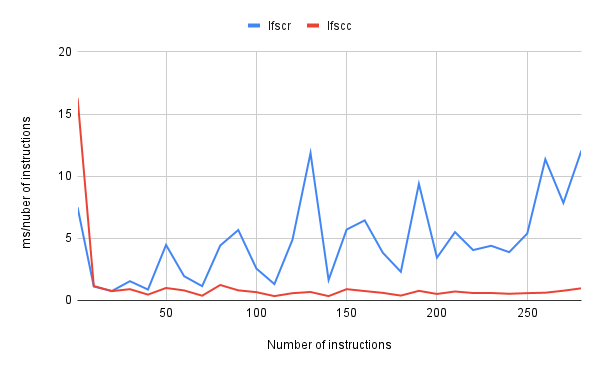
\includegraphics[width=0.7\textwidth]{chart2.png}
  \end{figure}
\end{frame}

\begin{frame}{Conclusion}
  \begin{itemize}
    \item Side Conditions might be unnecessary
    \item Formal verification of eBPF programs will take longer than the eBPF verifier
          but can be done fairly efficiently, but not with the approach tried in my work.
    \item Proposal is to take a similar approach to \textit{lfscc} and implement it in Rust, as it seems like a doable
          solution.
  \end{itemize}
\end{frame}

\end{document}